\documentclass[aps,prd,nofootinbib,twocolumn,reprint,superscriptaddress,showpacs,showkeys,longbibliography]{revtex4-1}
\pdfoutput=1
\usepackage{amsmath}
\usepackage{amssymb}
\usepackage{amsfonts}
\usepackage{amsthm}
\usepackage{mathrsfs}
\usepackage{natbib}
\usepackage{latexsym}
\usepackage{graphicx}
\usepackage{dsfont}
\usepackage{txfonts}
\usepackage{rotating}
\usepackage{wasysym}
\usepackage{multirow}
\usepackage{hhline}
\usepackage{graphicx}
\usepackage{hyperref}
\usepackage[dvipsnames,usenames]{color}
\usepackage{bm}
\usepackage{appendix}
\usepackage{acronym}
\usepackage{dcolumn}   % needed for some tables
\usepackage{enumitem}
\usepackage{bigdelim}
\usepackage{url}
\usepackage{caption}
\usepackage{subcaption}
\usepackage{multirow}
\usepackage{algorithm}
\usepackage[noend]{algpseudocode}
% REMINDER TO CHRIS: subcaption.sty might need to be included,
% or else the package removed; isn't universally installed -- GDM

\usepackage{framed}

%% ----- macros lifted from aastex.cls
\newcommand\arcdeg{\mbox{$^\circ$}}%
\newcommand\arcmin{\mbox{$^\prime$}}%
\newcommand{\bra}[1]{\langle #1|}
\newcommand{\ket}[1]{|#1\rangle}
\newcommand{\braket}[2]{\langle #1|#2\rangle}

%% ----- some handy shortcuts
\newcommand{\dcc}{LIGO-XXXXXXXXX}
%% -----
\newcommand{\cm}[1]{\textbf{\textcolor{red}{CM: #1}}}
\newcommand{\dg}[1]{\textbf{\textcolor{blue}{DG: #1}}}
%% ----- Version that makes the comments disappear
%% -----
\newcommand\marginnote[1]{%
    \mbox{}\marginpar{\raggedleft\hspace{0pt}\footnotesize\textcolor{green}
\raggedright\hspace{0pt}\footnotesize\textcolor{green}
    {#1}}}
%% ----- macros for cross-references

%% ----- input git-version tag
\input{tag.tex}

%% ----- define shorthand variables

\begin{document}

\title{Quantum matched filtering}

% NOTE TO EVERYBODY: we should decide on whether to make
% names full or initialized -- GDM
\author{Sijia Gao}
\email{s.gao.2@research.gla.ac.uk}
\affiliation{SUPA, School of Physics and Astronomy, University of Glasgow, Glasgow G12 8QQ, United Kingdom}
\author{Fergus Hayes}
\email{f.hayes.1@research.gla.ac.uk}
\affiliation{SUPA, School of Physics and Astronomy, University of Glasgow, Glasgow G12 8QQ, United Kingdom}
\author{Sarah Croke}
\affiliation{SUPA, School of Physics and Astronomy, University of Glasgow, Glasgow G12 8QQ, United Kingdom}
\author{J.~Veitch}
\affiliation{SUPA, School of Physics and Astronomy, University of Glasgow, Glasgow G12 8QQ, United Kingdom}
\author{C.~Messenger}
\affiliation{SUPA, School of Physics and Astronomy, University of Glasgow, Glasgow G12 8QQ, United Kingdom}

\date{\today}
\date{\commitDATE\\\mbox{\small{\commitID} \commitSTATUS}\\\mbox{\dcc}}

\begin{abstract}
We did a quantum thing
\end{abstract} 

\maketitle

\acrodef{NS}[NS]{Neutron Star}
\acrodef{GW}[GW]{gravitational-wave}

%%%%%%%%%%%%%%%%%%%%%%%%%%%%%%%%%%%%%%%%%%%%%%%%
%%%%%%%%%%%%%%%%%%%%%%%%%%%%%%%%%%%%%%%%%%%%%%%%
\section{Introduction}\label{sec:intro}

\begin{itemize}
\item GW introduction
\item Quantum computing introduction
\item summary of what this paper intends to do 
\end{itemize}

%%%%%%%%%%%%%%%%%%%%%%%%%%%%%%%%%%%%%%%%%%%%%%%%
%%%%%%%%%%%%%%%%%%%%%%%%%%%%%%%%%%%%%%%%%%%%%%%%
\section{Background}\label{sec:background}

\subsection{Matched-filtering}

Gravitational-wave signal searches require intensive data analysis techniques to detect as they are naturally weak signals and are buried in detector noise.
One advantage to the search is that the signal from binary sources is very well modeled; a gravitational wave form can be produced from numerical relativity given the binary systems parameters. 
Therefore the parameter space of interest can be discretized and a list of wave forms can be constructed as candidate signal \textit{templates}.
This list of wave forms we call the \textit{template bank}.
The selected points in the parameter space are spaced so that no more than $3\%$ of the maximum signal-to-noise ratio $\rho$ is lost due to the discretization \cite{capano2016implementing}.
Matched filtering is a signal processing technique used to determine a template that corresponds to the maximum $\rho$ out of the template bank.
The $\rho$ is calculated by correlating each template with the output from the detector.

\ \\
=======================================
\subsection*{Continuous}

For the derivation of a matched filter, consider the detector output to be $x(t)$, defined:

\begin{equation}
x(t) = s(t) + n(t),
\end{equation}

where $s$ is the signal combined with some zero-mean noise $n$.
Now consider a linear filter $q(t)$ that is applied to the data in the form of an inner product to enhance the signal component but reduce the noise.
Assuming the signal has some finite duration, this can be written in the frequency domain as:

\begin{equation}
q\cdot x = \int_{-\infty}^{\infty} \tilde{q}^{\ast}(f)\tilde{x}(f)df = \int_{-\infty}^{\infty} \tilde{q}^{\ast}(f)\tilde{s}(f)df + \int_{-\infty}^{\infty} \tilde{q}^{\ast}(f)\tilde{n}(f)df.
\end{equation}

It is evident that $q$ should be chosen as to maximize the inner product with the signal whilst minimizing the inner product with the noise.
Now we can define the output $\rho$ from these terms: 

\begin{equation}
\rho^{2} =  \frac{\left|\int_{-\infty}^{\infty} \tilde{q}^{\ast}(f)\tilde{s}(f)df\right|^{2}}
{\text{E}\left[\left|\int_{-\infty}^{\infty} \tilde{q}^{\ast}(f)\tilde{n}(f)df\right|^{2}\right]},
\end{equation}

for the case of zero-mean noise.
This can be rewritten:

\begin{equation}
\begin{split}
\rho^{2} = & \frac{\left|\int_{-\infty}^{\infty} \tilde{q}^{\ast}(f)\tilde{s}(f)df\right|^{2}}
{\text{E}\left[\int_{-\infty}^{\infty}\int_{-\infty}^{\infty} \tilde{q}^{\ast}(f)\tilde{q}(f')\tilde{n}^{\ast}(f')\tilde{n}(f)dfdf'\right]} \\ 
= & \frac{\left|\int_{-\infty}^{\infty} \tilde{q}^{\ast}(f)\tilde{s}(f)df\right|^{2}}
{\int_{-\infty}^{\infty}\int_{-\infty}^{\infty} \text{E}\left[\tilde{n}^{\ast}(f')\tilde{n}(f)\right]\tilde{q}^{\ast}(f)\tilde{q}(f')dfdf'} \\
= & \frac{\left|\int_{-\infty}^{\infty} \tilde{q}^{\ast}(f)\tilde{s}(f)df\right|^{2}}
{\int_{-\infty}^{\infty}\int_{-\infty}^{\infty} S_{n}(f)\delta(f-f')\tilde{q}^{\ast}(f)\tilde{q}(f')dfdf'} \\
= & \frac{\left|\int_{-\infty}^{\infty} \tilde{q}^{\ast}(f)\tilde{s}(f)df\right|^{2}}
{\int_{-\infty}^{\infty}S_{n}(f)|\tilde{q}(f)|^{2}df},
\end{split}
\end{equation}

where $S_n$ is the noise spectral density.
%We can use the Cauchy–Schwarz inequality to 
Expanding this once again:

\begin{equation}
\rho^{2} = \frac{\left|\int_{-\infty}^{\infty} \left(S_{n}^{1/2}(f)\tilde{q}(f)\right)^{\ast}\left(S_{n}^{-1/2}(f)\tilde{s}(f)\right)df\right|^{2}}
{\int_{-\infty}^{\infty}S_{n}(f)|\tilde{q}(f)|^{2}df}
\end{equation}

allows for an upper limit to be placed on $\rho$ using Cauchy-Schwarz inequality:

\begin{equation}
\left|\int_{-\infty}^{\infty} f^{\ast}(x)g(x)dx\right|^{2} \le \int_{-\infty}^{\infty}\left|f(x)\right|^{2}dx \int_{-\infty}^{\infty}\left|g(x)\right|^{2}dx,
\end{equation}

giving:

\begin{equation}
\begin{split}
\frac{\left|\int_{-\infty}^{\infty} \left(S_{n}^{1/2}(f)\tilde{q}(f)\right)^{\ast}\left(S_{n}^{-1/2}(f)\tilde{s}(f)\right)df\right|^{2}}
{\int_{-\infty}^{\infty}S_{n}(f)|\tilde{q}(f)|^{2}df} 
\\
\le
\frac{\int_{-\infty}^{\infty}S_{n}(f)|\tilde{q}(f)|^{2}df \int_{-\infty}^{\infty}S_{n}^{-1}(f)|\tilde{s}(f)|^{2}df}
{\int_{-\infty}^{\infty}S_{n}(f)|\tilde{q}(f)|^{2}df},
\end{split}
\end{equation}

constraining $\rho$ to:

\begin{equation}
\rho^{2} \le \int_{-\infty}^{\infty}S_{n}^{-1}(f)|\tilde{s}(f)|^{2}df.
\end{equation}

This upper bound is achieved when the template is equal to a noise-weighted copy of the signal:

\begin{equation}\label{equ:optsnr}
\tilde{q}(f) \propto \alpha\frac{\tilde{s}(f)}{S_n(f)}.
\end{equation}

In the case of gravitational-wave signal detection, the detector output is in the form of strain data sampled at a rate of 8192\,Hz, where the match filter of length $M$ is applied to the data via a convolution to give an estimate of the signal-to-noise ratio at a given data point $x[k]$:

\begin{equation}
\rho_i[k] = \sum_{i}^{M-1}h[i-k]x[k],
\end{equation}

where $h$ is the noise-weighted, time-reversed complex conjugate of a candidate signal as shown in Equation~\ref{equ:optsnr}.

\ \\
=======================================
\subsection*{Discrete}

In the case of gravitational-wave signal detection, the detector output is in the form of strain data sampled at a rate of 8192\,Hz.
For the derivation of a matched filter, consider the detector output to be a vector of length $M$ denoted $\vec{x}$, defined:

\begin{equation}
\vec{x} = \vec{s} + \vec{n},
\end{equation}

where $\vec{s}$ is the signal combined with some noise vector $\vec{n}$ with a mean of zero so that it has a covariance matrix $\vec{S}=\text{E}\left[\vec{n}\vec{n}^{\text{H}}\right]$.
Now consider a linear filter $\vec{q}$ that is applied to the data in the form of an inner product to enhance the signal component but reduce the noise.
Due to the filter's linearity, it can be written:

\begin{equation}
\vec{q}^{\text{H}}\vec{x} = \sum_{i=0}^{M-1} q^{\ast}[i]x[i] = \vec{q}^{\text{H}}\vec{s} + \vec{q}^{\text{H}}\vec{n}.
\end{equation}

It is evident that $\vec{q}$ should be chosen as to maximize the inner product with the signal whilst minimizing the inner product with the noise.
Now we can define the output SNR from these terms: 

\begin{equation}
\text{SNR}^{2} = \frac{|\vec{q}^{\text{H}}\vec{s}|^{2}}{\text{Var}\left[\sqrt{|\vec{q}^{\text{H}}\vec{n}|^{2}}\right]} = \frac{|\vec{q}^{\text{H}}\vec{s}|^{2}}{\text{E}\left[|\vec{q}^{\text{H}}\vec{n}|^{2}\right]},
\end{equation}

for the case of zero-mean noise.
This can be rewritten:

\begin{equation}
\begin{split}
\text{SNR}^{2} = & \frac{|\vec{q}^{\text{H}}\vec{s}|^{2}}{\text{E}\left[(\vec{q}^{\text{H}}\vec{n})(\vec{q}^{\text{H}}\vec{n})^{\text{H}}\right]} \\ 
= & \frac{|\vec{q}^{\text{H}}\vec{s}|^{2}}{\vec{q}^{\text{H}}\text{E}\left[\vec{n}\vec{n}^{\text{H}}\right]\vec{q}} = \frac{|\vec{q}^{\text{H}}\vec{s}|^{2}}{\vec{q}^{\text{H}}\vec{S}\vec{q}}.
\end{split}
\end{equation}



\begin{equation}
\text{SNR}^{2} = \frac{|(\vec{S}^{1/2}\vec{q})^{\text{H}}(\vec{S}^{-1/2}\vec{s})|^{2}}{(\vec{S}^{1/2}\vec{q})^{\text{H}}(\vec{S}^{1/2}\vec{q})}
\end{equation}

\ \\
=======================================

\begin{itemize}
\item derive matched-filtering as a semi-optimal statistic
\item What problem it solves
\end{itemize}

\subsection{Grovers algorithm}

The search for the closest matching template or templates in gravitational wave detection may be thought of as belonging to the class of generic search problems. For such problems, we wish to identify a ``marked" solution, i.e. one satisfying a certain set of criteria, from within an unstructured database of possible solutions. In fact, any problem for which it is easy to verify a solution, but difficult to find one may be thought of as a search problem, also known as NP problems. Indeed for certain NP-hard problems the best known classical algorithms offer limited improvement over brute-force search.\cite{bennett1997strengths} In the case of match filtering, we can consider the database to be made up of all possible templates, and we are searching for one or more for which the match with the data is above a specified threshold. Typically the number of templates is much larger than the complexity of checking whether a given template is a match, and is the limiting factor determining the time needed for match filtering in gravitational wave data analysis. For a database with $N$ entries and exactly one good solution, we need to check $\frac{N}{2}$ entries on average before finding the marked entry. In other words, for generic search problems, the required search time for a classical algorithm is $O(N)$ \cite{barnett2009quantum}. Grover's algorithm, proposed by Lov Grover in 1996, provides a polynomial speed-up for these problems, finding a solution in $O(\sqrt{N})$ search time \cite{grover1996fast}. It was later proved that this is asymptotically optimal; $\Omega(\sqrt{N})$ queries are required for a quantum algorithm to succeed with high probability \cite{bennett1997strengths}.
\newline\newline Grover's algorithm establishes a gap in query complexity between classical and quantum computers, in an oracle model. That is, it assumes that we have access to an oracle, a``black box" which computes a desired function, but not necessarily a description of the function itself. The query complexity is then given by the number of calls required to the oracle. To cast the search problem as an oracle problem, we can define a function $f(x)$, according to which $f(x)=1$ if and only if $x$ is our marked entry in the database, otherwise $f(x)=0$. In the quantum case, we imagine we have a quantum black box or oracle $U_f$ that can perform the following procedure:
\begin{equation}
    \label{Ufa}
    U_f: \ket{x}\otimes\ket{b}\longmapsto\ket{x}\ket{b \oplus f(x)},
\end{equation}
where $\ket{x}$ is the input register containing the input $x$ encoded as a computational basis state, and $\ket{b}$ is an ancilla register into which the output is written. We see that for $b=0$ the evaluation of the function is contained here. The key difference in the quantum case is that we can query the oracle in superposition, that is, we can prepare the input register in a superposition over all input states. In the rest of this section we outline Grover's algorithm, before addressing the problem of how to construct an oracle for match filtering in the following section. Grover's algorithm is covered in several introductory quantum computing texts, e.g. \cite{barnett2009quantum, nielsen2002quantum,kaye2007introduction}. We begin by noting that if we prepare our ancilla register in the state $\ket{-}=\frac{1}{\sqrt{2}}(\ket{0}-\ket{1})$, the operation given in Eq.~\ref{Ufa} is equivalent to the following procedure on the input register alone:
\begin{equation}
    \label{Uf}
    U_f: \ket{x}\longmapsto(-1)^{f(x)}\ket{x}.
\end{equation}
Although in the actual algorithm we need the ancilla register for the oracle, in the following discussion, we prefer to use Eq.~\ref{Uf} for the oracle evaluation for simplicity. 
\newline\newline Considering the problem of the search of the closest template, we represent the position of each template in the database as a computational basis state $\ket{i}$ and prepare the input register in an equal superposition over all positions $\ket{s}$. Suppose there are $N$ templates, the input register can be expressed as:
\begin{equation}
    \label{soo}
    \ket{s}=\frac{1}{\sqrt{N}}\sum^{N-1}_{0} \ket{i},
\end{equation}
where $\frac{1}{\sqrt{N}}$ represents the amplitude of each state in the superposition. This ensures that each state has the same probability of $\frac{1}{N}$ of being found. We shall start with the simplest situation where there is exactly one desired match, $\ket{w}$. The rest of the basis, i.e. the bad solutions can be marked as $\ket{s'}$, which are perpendicular to the state $\ket{w}$. We can rewrite the input state $\ket{s}$ using the new expression as:
\begin{equation}
    \label{so}
    \ket{s}=\frac{1}{\sqrt{N}}\ket{w}+\frac{\sqrt{N-1}}{\sqrt{N}}\ket{s'}.
\end{equation}
It is obvious that in order to decrease the number of enquiries needed to achieve the correct solution, we need to increase the amplitude of the state $\ket{w}$. We can also use a two dimensional vector graph to represent the input register $\ket{s}$ as shown in Fig.~\ref{2d0}A, where the angle is defined as:
\begin{equation}
\label{theta}
   \theta=\arcsin\braket{w|s}=\arcsin {\frac{1}{\sqrt{N}}}.
\end{equation}
Our goal, in the context, is to rotate state $\ket{s}$ to make it parallel, or closer to parallel, to state $\ket{w}$. After applying the oracle $U_f$, the input state $\ket{s}$ becomes:
\begin{equation}
    \label{ufs}
    U_f\ket{s}=-\frac{1}{\sqrt{N}}\ket{w}+\frac{\sqrt{N-1}}{\sqrt{N}}\ket{s'},
\end{equation}
which is equivalent to flip the input state $\ket{s}$ with respect to the horizontal axis $\ket{s'}$, as represented in Fig.~\ref{2d0}B. This procedure itself however, does not make the desired state $\ket{w}$ more favourable in the measurement. Therefore, an additional diffusion unitary operator is applied as the third step, which is defined as:
\begin{equation}
    \label{Us}
    U_s=2\ket{s}\bra{s}-\hat{\rm I},
\end{equation}
where $\hat{\rm I}$ is the identity operator. The action of this operator would result in the state:
\begin{equation}
    \label{usufs}
    U_sU_f\ket{s}=(1-\frac{4}{\sqrt{N}})\ket{s'}+\frac{1}{\sqrt{N}}(3-\frac{4}{N})\ket{w}.
\end{equation}
From Eq.~\ref{usufs} which it is obvious that the probability of $\ket{w}$ being the outcome of a measurement has increased from $\frac{1}{N}$ to $\frac{1}{N}(3-\frac{4}{N})^2$. This shows the speedup of Grover's algorithm as long as we have more than one template. If we decompose Eq.~\ref{ufs} into $\ket{s}$ and its orthogonal state, $\ket{s_\perp}$, as $U_f\ket{s}=a\ket{s}+b\ket{s_\perp}$, Eq.~\ref{usufs} can also be rewritten as:
\begin{equation}
    \label{usufsp}
    U_sU_f\ket{s}=a\ket{s}-b\ket{s_\perp}.
\end{equation}
This shows the diffusion operator is equivalent of flipping the $U_f\ket{s}$ state with respect to the $\ket{s}$ state, as shown in Fig.~\ref{2d0}C.
\begin{figure}[h]
{\caption{A) The red line represents the input initial state $\ket{s}$ represented as a vector in a plane spanned by the desired match $\ket{s}$ and undesired match $\ket{s'}$. B) The blue line represents the result of the oracle acting on the initial state $\ket{s}$ which now represented by the red dot dashed line. C) The green line represents the result of the diffusion operator acting on the result state in B, $U_f\ket{s}$ which now represented by the blue dotted line.   }\label{2d0}}
{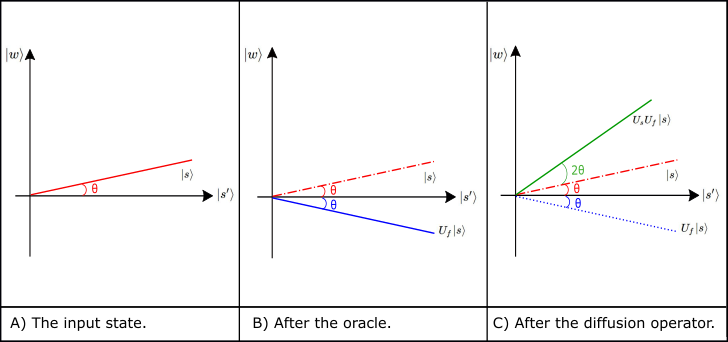
\includegraphics[width=0.45\textwidth]{Grover.png}}
 \end{figure}
If we define the grover operator $\hat{G}$ as:
\begin{equation}
    \label{Gdef}
    \hat{G}= U_sU_f,
\end{equation}
it is obvious from the previous discussion that it is equivalent to a rotation operator in the two-dimensional space spanned by $\ket{w}$ and $\ket{s'}$:
\begin{equation}
    \label{Gmatrix}
    \hat{G}=\begin{pmatrix}
\cos{2\theta} & \sin{2\theta} \\
-\sin{2\theta} & \cos{2\theta} 
\end{pmatrix}.
\end{equation}
After applying the Grover's operator $k$ times, the input state would become:
\begin{equation}
    \label{Gks}
    \hat{G}^k \ket{s}= \sin{\big((2k+1)\theta\big)}\ket{w}+\cos{\big((2k+1)\theta\big)}\ket{s'}.
\end{equation}
In order to maximise the probability of finding the desired match $\ket{w}$, we need to maximise its amplitude $\sin{\big((2k+1)\theta\big)}$. In other words, we need to apply the Grover's algorithm $k$ times that $(2k+1)\theta=\frac{\pi}{2}$. This means that:
\begin{equation}
\label{k}
    k\approx\frac{\pi}{4}\sqrt{N},
\end{equation}
for large number of templates.
\newline \newline
If there exists multiple matches, we can rewrite the input state $\ket{s_t}$ as:
\begin{equation}
    \label{som}
    \ket{s_t}=\sqrt{\frac{t}{N}}\ket{w_t}+\frac{\sqrt{N}-\sqrt{t}}{\sqrt{N}}\ket{s'_t},
\end{equation}
where $t$ is the number of desired templates, $\ket{w_t}$ refers to all the desired templates and $\ket{s'_t}$ are all the undesired templates. In this case, in the two-dimensional space spanned by $\ket{w_t}$ and $\ket{s'_t}$, state $\ket{s_t}$ is represented by a vector with an angle $\theta_t$ defined as:
\begin{equation}
\label{thetat}
   \theta_t=\arcsin\braket{w_t|s_t}=\arcsin {\sqrt{\frac{t}{N}}}. 
\end{equation}
Still, in order to maximise the amplitude of the desired templates, we need to apply the Grover's algorithm $k_t$ times that $(2k_t+1)\theta_t=\frac{\pi}{2}$. If the number $t$ of the desired templates are known, it is obvious that
\begin{equation}
\label{kt}
    k_t\approx\frac{\pi}{4}\sqrt{\frac{N}{t}}.
\end{equation}
However, in most cases we do not know the number of the desired templates. In this case we can use a variant of Grover's algorithm known as quantum counting\cite{brassard1998quantum}. As we have discussed above, each step in Grover's algorithm is a rotation through an angle $2 \theta_k$, which is now unknown. Quantum phase estimation is a well-known quantum algorithm which allows us to estimate just such an unknown angle of rotation. We don't describe this in detail here, but refer the interested reader to \cite{nielsen2002quantum}. For large number of templates N, the phase estimation part does not add extra complexity in the computation time \cite{brassard1998quantum}. In fact, it can find the period of a function in a time $O(log^3P)$, where P is a n-bit number representing the period. The extra computation time is polynomial in n.\cite{barnett2009quantum}

However, in most cases we do not know the number of the desired templates, t. %In this case we can use a variant of Grover's algorithm known as quantum counting
 Complementing Grover's algorithm with one of the most important subroutines in quantum computing, quantum phase estimation (QPE), quantum counting algorithm is able to produce the number of desired templates in the database and therefore determining the number of application of Grover's algorithm\cite{brassard1998quantum}.    
\newline\newline  Recall that we introduced the Grover's operator $\hat{G}$ as a rotation in the two-dimension space spanned by $\ket{w_t}$ and $\ket{s'_t}$ in Eq.\ref{Gmatrix}, the eigenvectors for it would be:
\begin{equation}
  \label{Geigenvector}  
    \ket{s_+}=\begin{pmatrix}
\frac{i}{\sqrt{2}} \\
\frac{1}{\sqrt{2}}
\end{pmatrix}, \qquad
\ket{s_-}=\begin{pmatrix}
\frac{-i}{\sqrt{2}} \\
\frac{1}{\sqrt{2}}
\end{pmatrix},
\end{equation}
with eigenvalues of $e^{i2\theta_t}$ and $e^{-i2\theta_t}$ respectively. Therefore the problem of finding the number of the desired templates is transformed to a eigenvalue estimation problem, which is what QPE designed to solve.  
\newline \newline A set of integers ranging from  $0$ to $2^P-1$ can be represented by P qubits as:
\begin{equation}
    \label{H0N}
    \hat{H}^P\ket{0}=\frac{1}{2^{\frac{P}{2}}}(\ket{0}+\ket{1})\otimes...\otimes(\ket{0}+\ket{1})=\sum_{a=0}^{2^P-1}\ket{a},
\end{equation}
which inspires a new set of computational basis $\ket{\Tilde{b}}$ using quantum Fourier transform (QFT)\cite{coppersmith2002approximate}:
\begin{equation}
\begin{split}
   \label{QFT}
    \ket{\Tilde{b}}=\hat{U}_{QFT}\ket{b}&=\sum_{a=0}^{2^P-1}e^{i\frac{2\pi ab}{2^P}}\ket{a}\\
    &=\frac{1}{2^{\frac{P}{2}}}(\ket{0}+e^{i\pi b}\ket{1})\otimes(\ket{0}+e^{i\frac{\pi b}{2}}\ket{1})\otimes...\otimes(\ket{0}+e^{i\frac{\pi b}{2^{P-1}}}\ket{1}).
\end{split}
\end{equation}
This motivated us to use the counting register as a control register to apply controlled Grover's gate to the input state:
\begin{equation}
\begin{split}
   \label{CG}
    \sum_{a=0}^{2^P-1}C\text{-}\hat{G}^a\ket{a}\otimes \ket{s_t}&=\sum_{a=0}^{2^P-1}e^{i2\theta_t a}\ket{a}\otimes\ket{s_t}\\
    &=\frac{1}{2^{\frac{P}{2}}}(\ket{0}+e^{i2\theta_t }\ket{1})\otimes(\ket{0}+e^{i2\theta_t2^1}\ket{1})\otimes...\otimes(\ket{0}+e^{i2\theta_t2^{P-1}}\ket{1})\otimes\ket{s_t}.
\end{split}
\end{equation}
Comparing Eq.~\ref{QFT} and Eq.~\ref{CG}, we naturally proceed to apply an inverse QFT to Eq.~\ref{CG} to extract the eigenvalue $\theta_t$ containied in the phase information:
\begin{equation}
   \label{InverQFT}
   \hat{U}^{-1}_{QFT}\sum_{a=0}^{2^P-1}e^{i2\theta_t a}\ket{a}\otimes\ket{s_t}=\frac{1}{2^{P}}\sum_{a=0}^{2^P-1} \sum_{b=0}^{2^P-1} e^{i2\pi a(\frac{\theta_t}{\pi}-\frac{b}{2^P})}\ket{b}\otimes\ket{s_t}.%this part can elaborate in thesis according to steve's 7.38
\end{equation}
Within the basis $\{\ket{b}\}$, the states $\ket{b}$ satisfies $\frac{\theta_t}{\pi}-\frac{b}{2^P}=0$ or $\frac{\pi -\theta_t}{\pi}-\frac{b}{2^P}=0$ would be the most probable states in the measurement. Even in situations that $\frac{\theta_t}{2^P\pi}$ is not an integer, the system would still peak near the state $b=\frac{\theta_t}{2^P\pi}$. In fact, according to the original quantum counting paper by Brassard \cite{brassard1998quantum}, with no less than 4 counting qubits, we can achieve an output with an error less than $\frac{2\pi}{P}\sqrt{t}+\frac{\pi^2}{P^2}$ with a probability of at least $\frac{8}{\pi^2}$. In order to obtain an outcome with an error probability less than $\frac{1}{2^P}$, %get how this is proved
we should evaluate the counting algorithm l times, which is in O(P). From Eq.~\ref{thetat}, in order to differentiate between $|\tilde{t}-t|=1$, P needs to be chosen such that:
\begin{equation}
    \label{P}
    \frac{1}{2^P}\leq \frac{\sqrt{t}-\sqrt{t-1}}{\sqrt{N}\pi}\approx \frac{1}{\sqrt{Nt}\pi}.
\end{equation}


%%%%%%%%%%%%%%%%%%%%%%%%%%%%%%%%%%%%%%%%%%%%%%%%
%%%%%%%%%%%%%%%%%%%%%%%%%%%%%%%%%%%%%%%%%%%%%%%%
\section{Quantum psuedo-code}\label{sec:psuedocode}
In the previous section we introduced Grover's algorithm and quantum phase estimation algorithm, and how, in principle, they can speed up the process of searching for one or more desired matches in gravitational wave research. In this section we are going to present the pseudo code of this implementation and prove that we can effectively construct the required oracle. We will also present relevant calculation and compare it with the classical cost to prove the speed up.
\newline \newline In the quantum circuit implementation, we only use C-X gate and other one qubit gates. Our initial assumption being all these gates have the same computational cost, with which estimating the overall computational cost is the same as counting the number of gates. Suppose there are N templates. Classically, for each template we suppose it takes $k_1$ steps to compute a template from its parameters, $k_2$ steps to match the template to the data and $k_3$ steps to compare the result with the threshold to determine if this template is desirable. In this way, to match all templates we need $N \cdot (k_1+k_2+k_3)$ steps, which is the total cost. As for $k_1$ and $k_2$, they should be polynomial to the size of the data D, therefore possessing a complexity of O(D), and $k_3$ should be polynomial to the size of the threshold T that we are comparing the result of the match to, which is a constant, Therefore, its complexity should be O(1). Consequently, the total computational complexity of the classical algorithm should be O(D*N).  
\newline \newline The quantum search algorithm we will present is based on Grover's algorithm and quantum phase estimation. In Algorithm.~\ref{GroGate}, we present the pseudo code to construct the Grover's gate, in which we give an example of how to construct an oracle that performs template matching that tolerates noise. In Algorithm.~\ref{GroPseudo}, we present the pseudo code performs the search algorithm in a database with multiple templates matching the data utilising the Grover's gate. The fact that our algorithm carries out the search on the index rather than the templates means it is efficient and the amount of search qubits need only depends on the number of templates rather than the size of the templates.
\begin{algorithm}[H]
\caption{Grover's Gate}\label{GroGate}
\begin{algorithmic}[1]
\Function{Grover's Search algorithm}{N, $\ket{Data}$}
\label{GroverPseudo}
\Procedure{Oracle Construction}{}
\State \emph{Creating templates}:
\ForAll{$i<N$}
    \State{$ \ket{i}\ket{0} \gets \ket{i}\ket{T_i}$}
\EndFor
\State \emph{Comparison with the data}:
    \State$\ket{i}\ket{Data}\ket{T_i}\ket{0} \gets \ket{i}\ket{Data}\ket{T_i}\ket{F(i)}$
        \If {$F(i) <  Threshold$}
            \State $f(i)=0$
        \Else 
            \State $f(i)=1$
       %\State \textbf{close};
        \EndIf
\State $\ket{i}\ket{Data}\ket{T_i}\ket{F(i)} \gets (-1)^{f(i)}\ket{i}\ket{Data}\ket{T_i}\ket{F(i)} $
\State \emph{Dis-entangling registers}:
    \State $(-1)^{f(i)}\ket{i}\ket{Data}\ket{T_i}\ket{F(i)} \gets (-1)^{f(i)}\ket{i}\ket{Data}\ket{T_i}\ket{0}$
    \State $(-1)^{f(i)}\ket{i}\ket{Data}\ket{T_i}\ket{0}\gets (-1)^{f(i)}\ket{i}\ket{0}\ket{Data}\ket{0}$
\EndProcedure
\Procedure{Diffusion Operator}{}
\State $ \sum(-1)^{f(i)}\ket{i}  \gets \sum(2\ket{i}\bra{i}-\hat{\rm I})(-1)^{f(i)}\ket{i}$
\EndProcedure
\EndFunction
\end{algorithmic}
\end{algorithm}
\textbf{Discussion:} For Algorithm. \ref{GroGate}, the following is the explanation for each step and the related computational cost.
\begin{itemize}
    \item Step 0: The original state would be comprised of four registers:
        \begin{equation}
            \label{step0}
            \frac{1}{\sqrt{N}}\sum^N_i\ket{i}_I\ket{0}_T\ket{Data}_D\ket{+}_A,
        \end{equation}
        the subscripts I, T, D and A represents the indices, the templates, data and the ancilla for Grover's algorithm respectively. 
    \item  \textbf{Oracle construction:} 
        \begin{itemize}
             \item Step 1: Creating templates. Cost: $k_1$
               \newline We assume for each template this should be the same cost as the classical computer. However, since all the calculation can be done in parallel, the cost would only be $k_1$. The state after this step would be:
                \begin{equation}
                \label{step1}
                \frac{1}{\sqrt{N}}\sum^N_i\ket{i}_I\ket{T_i}_T\ket{Data}_D\ket{+}_A,
                \end{equation}
            \item Step 2: Comparison with the data. Cost: $k_2+k_3$
             \newline We assume for each template this step should cost the same as the classical algorithm. However, since all templates are stored in superposition, all the calculation can be done in parallel, and the result $F(i)$ is stored in a separate register. The cost of calculating the overlap between the templates and the data would be the same as the classical case, $k_2$. However, in order to use the Grover's algorithm, we need to compare this result with a threshold to determine if we should add 1 or 0 to the ancilla. This threshold is predetermined, on account for precision and noise tolerance. After we register the result on the ancilla, which would incur a cost of $k_3$. The state after this step would be: 
            \begin{equation}
                \label{step2}
                \frac{1}{\sqrt{N}}\sum^N_i(-1)^{f_i}\ket{i}_I\ket{T_i}_T\ket{Data}_D\ket{+}_A\ket{F_i},
            \end{equation}
            where $f(T_i)$ denotes if the overlap between the templates and the data is above the threshold.
            \item Step 3: Disentangling registers. Cost: $k_1+k_2$.
            \newline In order to carry out the Grover's algorithm we need only the indices. Therefore, the register holding the result of the overlap $F_i$ needs to be erased. The erasing process is the reverse of the generating process. Accordingly, another $k_2$ cost is generated. In the reversion, the template register is stored, which needs to be erased as well. Accordingly, $k_1$ cost is generated. The state after this step would be: 
            \begin{equation}
            \label{step3}
            \frac{1}{\sqrt{N}}\sum^N_i(-1)^{f_i}\ket{i}_I\ket{0}_T\ket{Data}_D\ket{+}_A,
            \end{equation}
        \end{itemize}
   \item  Step 4: Diffusion Operator. Cost: $34(\log_2 N)-31$. 
        \newline This step is a unique step in the quantum algorithm so its cost would be calculated using gate costs. The diffusion operator is acting on the equal superposition of the index register, made up of Hadmard gates acting on all the qubits twice with a $C^{\log_2 N-1}$-$Z$ gate in the middle. For $N$ templates, $\log_2 N$ qubits is needed. Therefore, there are $2\log_2 N$ Hadmard gates in the diffusion operator. A $C^{\log_2 N-1}$-$Z$ gate can be decomposed into $32(\log_2 N-1)+1$ gates only using C-X gates and one qubit gates. Therefore, there are in total $(34(\log_2 N)-31)$ gates involved. The cost would be in the order of $\log_2 N$. 
    \item Total cost: $2k_1+2k_2+k_3+34(\log_2 N)-31$
\end{itemize}

\begin{algorithm}[H]
\caption{Grover's algorithm implementation on template searching}\label{GroPseudo}
\begin{algorithmic}[1]
\State $\textit{P} \gets \text{number of }\textit{precision digits}$
\State $\textit{N} \gets \text{number of }\textit{templates}$
\State $i \gets \text{index of} \textit{ templates}$
\State $\textit{l} \gets \text{number of repetition of quantum phase estimation}$
\State \emph{Creating templates}:
\ForAll{$i<N$}
\State{$ \ket{i}\ket{0} \gets \ket{i}\ket{T_i}$}
\EndFor

\Procedure{Quantum Phase estimation}{n}
\label{QPE}
\State \emph{Creating the counting register }:
\State{$ \ket{i}\ket{T_i}\gets \ket{0}^P\ket{i}\ket{T_i}$}
\State{$ \ket{0}^P\ket{i}\ket{T_i}\gets \frac{1}{2^{P/2}}(\ket{0}+\ket{1})^P\otimes\ket{i}\ket{T_i}$}
\State \emph{Controlled Grover' gate}:
\ForAll{$a<2^P$}
   \State $j \gets a$
    \Repeat
        \State Algorithm.\ref{GroGate} \Call{Grover's Gate}{N, $\ket{Data}$}, $j--$
    \Until{$j==0$}
\EndFor
\State$\frac{1}{2^{P/2}}(\ket{0}+\ket{1})^n\otimes\ket{i}\ket{T_i} \gets \frac{1}{2^{P/2}}\sum e^{2i\theta_t a}\ket{a}\otimes\ket{i}\ket{T_i} $
\State \emph{Inverse Quantum Fourier Transform}:
    \State$\frac{1}{2^{P/2}}\sum e^{2i\theta_t a}\ket{a}\otimes\ket{i}\ket{T_i}\gets \frac{1}{2^{P}}\sum \sum e^{2\pi a i(\frac{\theta_t }{\pi}-\frac{x}{2^P})}\ket{x}\otimes\ket{i}\ket{T_i}$
\State \emph{Measurement}:
    \State$x-\frac{2^P\theta_t }{\pi}=0 $ %constructive interference across all m
\State \emph{Output}:
    \State$\frac{\theta_t }{\pi}\gets\frac{x}{2^P} $
%$(2k_t+1)=\frac{\pi}{2\theta_t}$ $k_t=\frac{\pi}{4\theta_t}-1/2$
\State $k_t \gets \textbf{Floor}[\frac{2^P}{4x}-\frac{1}{2}]$
\EndProcedure
\Repeat 
    \State  \Call{Quantum Phase estimation}{n}, $l--$
    \State  $Array~\{k_t(l)\} \gets k_t$
\Until{$l==0$}
\State $k_t \gets \textbf{Mode}{\{k_t(l)\}}$
\Procedure{Search}{}
    \Repeat
        \State Algorithm.\ref{GroGate} \Call{Grover's Gate}{N, $\ket{Data}$}, $k_t--$
    \Until{$k_t==0$}
    \State \emph{Output}:
    \State $i_{correct}$
\EndProcedure
\end{algorithmic}
\end{algorithm}
\textbf{Discussion:} For Algorithm. \ref{GroPseudo}, the following is the explanation for each step and the related computational cost.
\begin{itemize}
    \item Step 0:  This is the same as the step 0 in Algorithm.~\ref{GroverPseudo}.
    \item Step 1: Creating templates. Cost: $k_1$
               \newline This is the same as the step 1 in Algorithm.~\ref{GroverPseudo}.
    \item  \textbf{Quantum phase estimation:} 
        \begin{itemize}
        \item Step 2: Creating counting register. Cost: $P$ 
        \newline This step involves applying Hadmard gate to each qubit. There are n counting qubits. Therefore the cost would be n. The state after this step would be:
                \begin{equation}
                \label{step2}
                \frac{1}{2^{P/2}}(\ket{0}+\ket{1})^P\otimes\ket{i}\ket{T_i},
                \end{equation}
        The precision parameter P
        \item Step 3: Controlled Grover's Gate. Cost: $(2k_1+2k_2+k_3+34(\log_2 N)-31)*2^{P}$ 
        \newline In this step, we are applying the Grover's gate i times to state $\ket{i}$. The total number of application is $\sum^{2^P-1}_{i=0} i=2^P$ times. The state after this step would be:
                \begin{equation}
                \label{step3A2}
                \frac{1}{2^{P/2}}\sum e^{2i\theta_t a}\ket{a}\otimes\ket{i}\ket{T_i},
                \end{equation}
        \item Step 4: Inverse quantum Fourier transform. Cost: $P^2$ \cite{barnett2009quantum}
        \item Step 5: Measurement. Cost: $P$
        \newline The cost of measurement should be $1$ for each counting qubit.
        \item Step 6: Output. Cost: 1
        \item Step 7: Repeat Quantum phase estimation. \newline Cost: $l*((2k_1+2k_2+k_3+34(\log_2 N)-31)*2^{P}+P+P^2+1.5)$
        \newline Because quantum phase estimation output the ideal number of repetition with a probability. In order to achieve a sufficiently convincing result we need to run the algorithm a number of times: which we set as $l$, that is irrelevant to the data and template sizes. Every time we store the $k_t(i)$ into an array and the number that appeared the most times would be the $k_t$ we shall use in the search step. The process of finding the modal number in the array $k_t(i)$ is recorded as $l/2$ times as an average search time.
        \end{itemize}
    \item Step 7: Search. Cost: $(2k_1+2k_2+k_3+34(\log_2 N)-31)*\sqrt{\frac{N}{t}}$
    \newline Grover's algorithm shall be repeated $k_t$ times to achieve the desired template index. $k_t$ according to our previous discussion should be $O(\sqrt{\frac{N}{t}})$.
    \item Total Cost: $(2k_1+2k_2+k_3+34(\log_2 N)-31)*(l*2^{P}+\sqrt{\frac{N}{t}})+l*(P+P^2+1.5)$
\end{itemize}
According to the discussion in Section.~\ref{quantc}, the complexity of l is $O(P)$, and P is of complexity  $O(log(\sqrt{Nt}))$. Therefore, the overrall complexity of the quantum algorithm is $O\Big((D+logN)\big(log(\sqrt{Nt})\sqrt{Nt}+\sqrt{\frac{N}{t}}\big)+log^2(\sqrt{Nt}))\Big)$. In the case where the number of matching templates is small comparing with the the library of the templates, we can simplify the complexity into $O\big(\sqrt {N} logN(D+logN)\big)$, which is smaller than the classical complexity of $O(DN)$ when the data size and template size are all big. In gravitational wave template searching, it normally involves $10^4$ to $10^{12}$ templates, \sjg{quotes from Chris, but reference needed here}. with the lower bound of the number of templates, $10^4$, P and l can be chosen at 7. In the classical case, the computational cost is approximately $O(10^4)$; in the quantum case, the computational cost is approximately $\Omega(10^3)$. There is an order of magnitude difference even for the smallest number of cases. In general, it is safe to conclude that our quantum algorithm offers a $\sqrt{N}$ speed up with a practical oracle.



%%%%%%%%%%%%%%%%%%%%%%%%%%%%%%%%%%%%%%%%%%%%%%%%
%%%%%%%%%%%%%%%%%%%%%%%%%%%%%%%%%%%%%%%%%%%%%%%%
\section{Example using Qiskit}\label{sec:qizkitexample}

\begin{itemize}
\item define model (small number of qubits and exact matching)
\item one template matching
\item multiple templates matching
\item focus on results
\item run on the actual quantum processor and compare the results, efficiency and gate costs
\end{itemize}

%%%%%%%%%%%%%%%%%%%%%%%%%%%%%%%%%%%%%%%%%%%%%%%%
%%%%%%%%%%%%%%%%%%%%%%%%%%%%%%%%%%%%%%%%%%%%%%%%
\section{Example on Sine wave (python)}\label{sec:sineexample}

\begin{itemize}
\item continuous wave GW signal motivation
\item why we don't just use the QFT? Our real CW signals (and CBCs) are not monochromatic
\item Define sine wave model
\item focus on showing results - number of steps taken
\end{itemize}

%%%%%%%%%%%%%%%%%%%%%%%%%%%%%%%%%%%%%%%%%%%%%%%%
%%%%%%%%%%%%%%%%%%%%%%%%%%%%%%%%%%%%%%%%%%%%%%%%
\section{CBC application example}\label{sec:cbcexample}

\begin{itemize}
\item define the CBC waveform model
\item focus on results - compare to GWOSC GW150914 data
\item make the number of steps clear (~ root N operations)
\end{itemize}

%%%%%%%%%%%%%%%%%%%%%%%%%%%%%%%%%%%%%%%%%%%%%%%%
%%%%%%%%%%%%%%%%%%%%%%%%%%%%%%%%%%%%%%%%%%%%%%%%
\section{Practical considerations}\label{sec:praccon}

Discuss things about practicalities for the future. How many qubits are needed
etc.. 

\begin{itemize}
\item space requirements on quantum computer
\item describe the current state of the art in quantum processors
\end{itemize}

%%%%%%%%%%%%%%%%%%%%%%%%%%%%%%%%%%%%%%%%%%%%%%%%
%%%%%%%%%%%%%%%%%%%%%%%%%%%%%%%%%%%%%%%%%%%%%%%%
\section{Discussion}\label{sec:discussion}

\begin{itemize}
\item Summarise the entire paper first
\item highlight the parts of interest to Quantum and GW fields separately
\item Discuss limitations of what we've done
\item Talk about future work
\item Talk about the future of Quantum computers and the future GW data
analysis challenges
\item It's not just GWs though - data analysis searches in general
\end{itemize}

%%%%%%%%%%%%%%%%%%%%%%%%%%%%%%%%%%%%%%%%%%%%%%%%
\begin{acknowledgments}
We would liek the thank \ldots
\end{acknowledgments}


%%%%%%%%%%%%%%%%%%%%%%%%%%%%%%%%%%%%%%%%%%%%%%%%
\appendix

%%%%%%%%%%%%%%%%%%%%%%%%%%%%%%%%%%%%%%%%%%%%%%%%
%%%%%%%%%%%%%%%%%%%%%%%%%%%%%%%%%%%%%%%%%%%%%%%%
\section{Optional Appendix\label{sec:appendix}}


% Create the reference section using BibTeX:
\bibliography{masterbib}

\end{document}